\subsection{Resultados do Bosque}
\label{resultados_bosque}
Neste momento, serão mostrados os resultados das execuções baseadas no BOSQUE.

\subsubsection{Treinamento} \label{result_treino_bosque}
Na Tabela \ref{tab:resultados_treino_bosque}, vemos os resultados dos treinamentos do SP sobre Bosque transduzido por nós. Note que os campos são equivalentes aos explicados em \ref{result_treino_cintil}.
\begin{center}
    \begin{table}[h!]
    \centering
    % \begin{tabular}{|l|c|c|c|c|c|c|}
    % \hline
    %     Grammar & States & Tags & Words & UnaryR & BinaryR & Taggings\\
    %     \hline
    %     1 & 482 & 15 & 2881 & 59 & 1182 & 2948\\
    %     2 & 496 & 16 & 2627 & 66 & 1170 & 2679\\
    %     3 & 527 & 16 & 2845 & 52 & 1206 & 2902\\
    %     4 & 505 & 17 & 2779 & 67 & 1188 & 2841\\
    %     5 & 480 & 16 & 2649 & 59 & 1166 & 2705\\
    %     6 & 487 & 16 & 2847 & 53 & 1190 & 2900\\
    %     7 & 472 & 15 & 2774 & 54 & 1192 & 2825\\
    %     8 & 477 & 17 & 2823 & 66 & 1192 & 2889\\
    %     9 & 522 & 18 & 2718 & 64 & 1183 & 2778\\
    %     10 & 404 & 16 & 2559 & 50 & 1027 & 2614\\
    %     \hline
    % \end{tabular}
    \csvautotabular{tabelas/resultados-bosque-treino.csv}
    \caption[Resultados do treinamento do Bosque]{Resultados dos treinamentos do Bosque, para os 10 \textit{folds}}
    \label{tab:resultados_treino_bosque}
\end{table}
\end{center}

A Figura \ref{fig:treino_bosque} nos dá a visualização desses resultados. Pode-se observar que o resultado pre-eliminar dos testes é muito superior ao visualizado em \ref{result_treino_cintil}.
\begin{center}
    \begin{figure}[!ht]
    \centering
    % \includegraphics{}
    \includesvg[width=.8\textwidth]{imagens/treino_bosque}
    % \includesvg{imagens/bosque_pcfg}
    \caption[Gráfico de resultados do treinamento, usando o BOSQUE transduzido]{Gráfico de resultados do treinamento do LexicalizedParser, usando o BOSQUE transduzido}
    \label{fig:treino_bosque}
\end{figure}
\end{center}

\subsubsection{Avaliação} \label{result_aval_bosque}
Na Tabela \ref{tab:result_bosque_pcfg}, vemos o resultados dos testes utilizando o SP sobre o Bosque transduzido.
\begin{center}
    \begin{table}[!h]
    \centering
    \begin{tabular}{|l|c|c|c|}
        \hline
        % pcfg LP/LR summary evalb    &   LP  & LR    &   F1\\
        pcfg LP/LR & LP & LR & F1\\
        \hline
        fold 1 & 51.61 & 47.9 & 49.69\\
        fold 2 & 51.78 & 47.68 & 49.64\\
        fold 3 & 49.25 & 45.65 & 47.38\\
        fold 4 & 52.55 & 49.05 & 50.74\\
        fold 5 & 51.03 & 46.05 & 48.41\\
        fold 6 & 52.8 & 49.15 & 50.91\\
        fold 7 & 48.86 & 45.21 & 46.97\\
        fold 8 & 50.1 & 45.81 & 47.86\\
        fold 9 & 52.28 & 48.49 & 50.32\\
        fold 10 & 55.37 & 51.91 & 53.59\\
        \hline
    \end{tabular}
    % \csvautotabular{resultados-cintil-testes-pcfg.csv}
    \caption{Resultados do treinamento da PCFG do SP, usando dados do BOSQUE}
    \label{tab:result_bosque_pcfg}
\end{table}
% fold 1   &   44.6    &   41.62   &   43.06\\
% fold 2   &   44.15   &   41.48   &   42.78\\
% fold 4   &   44.52   &   41.4   &   42.9\\
% fold 5   &   44.17   &   41.56   &   42.82\\
% fold 6   &   44.29   &   41.02   &   42.59\\
% fold 7   &   44.92   &   42.14   &   43.49\\
% fold 8   &   44.83   &   41.62   &   43.17\\
% fold 9   &   43.88   &   40.83   &   42.3\\
% fold 10   &   43.78   &   40.54   &   42.1\\
\end{center}

A média da \textit{F1-Score} é de 49.551\%, e tem o desvio padrão de aprox. 1.992\%.

Na Figura \ref{fig:bosque_result_pcfg} podemos ter uma visualização melhor de tais resultados.
\begin{center}
    \begin{figure}[!ht]
    \centering
    % \includegraphics{}
    \includesvg[width=.8\textwidth]{imagens/bosque_pcfg}
    % \includesvg{imagens/cintil_pcfg}
    \caption[Gráfico de resultados dos testes usando o BOSQUE transduzido]{Gráfico de resultados dos testes do PCFG do LexicalizedParser, usando o BOSQUE transduzido}
    \label{fig:bosque_result_pcfg}
\end{figure}
\end{center}

É possível notar que, mesmo com o desempenho de treinamento melhor que os do CINTIL (como visto em \ref{result_treino_cintil}), a classificação continua tendo uma qualidade baixa. 
% nunca superando os 50\%.
Apenas os dois últimos \textit{folds} superam os 50\%.

\subsubsection{Estudos de caso}
\label{subsec:ec-bosque}

De modo análogo ao do CINTIL, vamos revisar aqui alguns casos curiosos de sentenças classificadas. Utilizaremos a gramática do décimo treino para as classificações e avaliações. O Bosque tem mais casos problemáticos que o CINTIL, e visualizar todas elas tornaria este trabalho ainda maior. Portanto, alguns casos serão exibidos apenas nos Apêndices.
\begin{center}
    \begin{figure}[!ht]
    \centering
    % \includegraphics{}
    \begin{minipage}{.45\textwidth}
        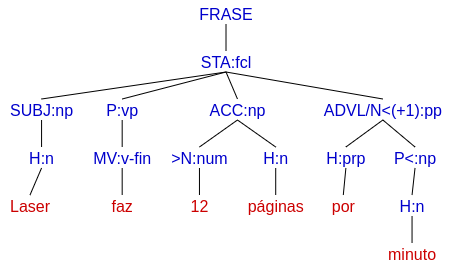
\includegraphics[width=\linewidth]{imagens/ec_bosque_sem_ponto_tree_orig.png}
        \caption{árvore original}
    \end{minipage}
    % 
    \begin{minipage}{.45\textwidth}
        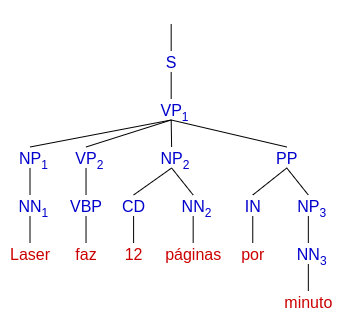
\includegraphics[width=\linewidth]{imagens/ec_bosque_sem_ponto_tree_trans.png}
        \caption{árvore transduzida}
    \end{minipage}
    \begin{minipage}{.45\textwidth}
        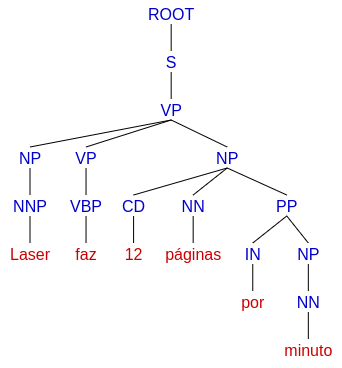
\includegraphics[width=\linewidth]{imagens/ec_bosque_sem_ponto_tree_sp.png}
        \caption{árvore gerada pelo SP}
    \end{minipage}
    \caption[Estudo de caso BOSQUE - Sentença transduzida sem pontuação]{Estudo da sentença CF761-1, \textquote{Laser faz 12 páginas por minuto}, que originalmente não possui nenhuma pontuação}
    \label{fig:ec_bosque_sem_ponto_tree}
\end{figure}
\end{center}

A Figura \ref{fig:ec_bosque_sem_ponto_tree} nos mostra as diferenças entre árvores sem pontuação. Foram removidas as informações adicionais dos nós da árvore original do Bosque, mantendo apenas $(F:f)$.
Temos poucos erros de \textit{parsing}. Nenhum nó terminal foi classificado erroneamente, apenas nós internos (não-terminais). Uma ambiguidade no $NP$ de \textquote{12 páginas}, que agora abarca também o $PP$ irmão. 
% E o núcleo do primeiro $NP$, que foi classificado como $NP$.

\begin{center}
    \begin{figure}[!hb]
    \centering
    % \includegraphics{}
    \begin{minipage}{.45\textwidth}
        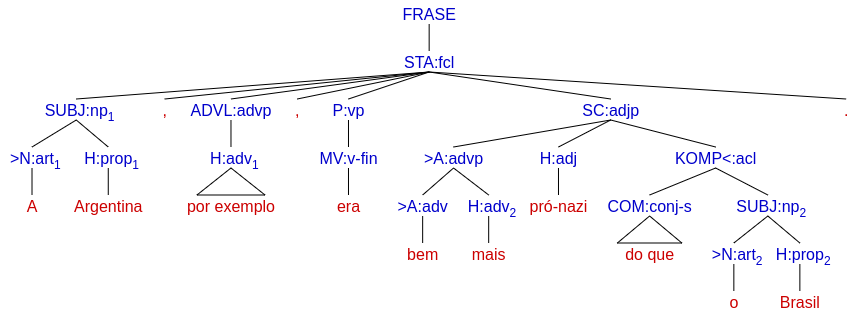
\includegraphics[width=\linewidth]{imagens/ec_bosque_komp_tree_orig.png}
        \caption{árvore original}
    \end{minipage}
    % 
    \begin{minipage}{.45\textwidth}
        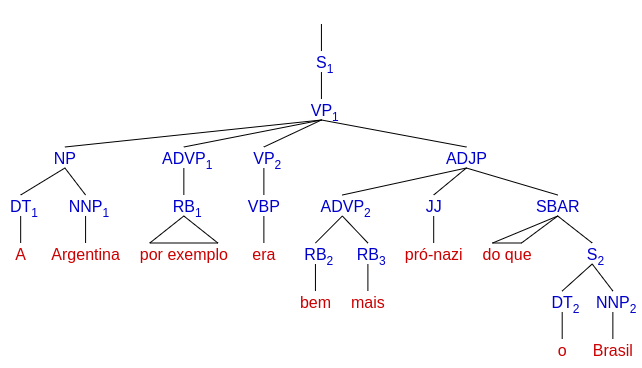
\includegraphics[width=\linewidth]{imagens/ec_bosque_komp_tree_trans.png}
        \caption{árvore transduzida}
    \end{minipage}
    \begin{minipage}{.45\textwidth}
        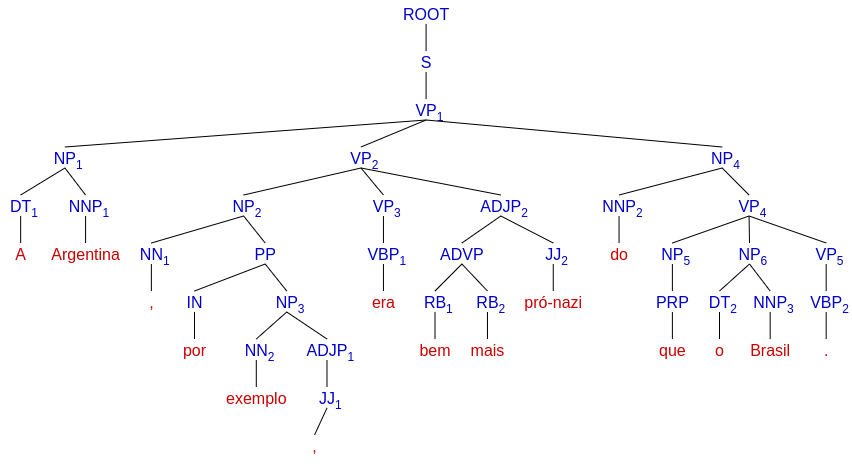
\includegraphics[width=\linewidth]{imagens/ec_bosque_komp_tree_sp.png}
        \caption{árvore gerada pelo SP}
    \end{minipage}

    \caption[Estudo de caso BOSQUE - Sentença transduzida com KOMP<:acl]{Estudo da sentença CF766-10, \textquote{A Argentina, por exemplo, era bem mais pró-nazi do que o Brasil.}, que possui a estrutura KOMP<:acl internamente.}
    \label{fig:ec_bosque_komp_tree}
\end{figure}
\end{center}

A Figura \ref{fig:ec_bosque_komp_tree} traz uma sentença que, originalmente, possui o par $KOMP<:acl$ internamente. É notório como as regras unárias (Não-terminal $\rightarrow$ terminal) são mais consistentes que as binárias. Curioso também a separação de palavras originalmente conjuntas, como \textquote{por exemplo} e \textquote{do que}. Ambas expressões aparecem pouco no CETEMFolha (22 e 34 vezes, respectivamente). Porém, pelas observações anteriores, supõe-se que o SP não está pronto para lidar com nós terminais concatenados durante a execução. 
% Cabe observar que a estrutura de Comparação foi mantida no estilo PTB, como visto em \ref{fig:ec_bosque_komp_detalhe}, apesar da discordância entre $SBAR$ (transdução) e $PP$ (\textit{Stanford}).
Interessante notar que a estrutura de Comparação (estudada em \ref{subsec:tag_komp}) foi desfeita pelo SP.

\begin{center}
    \begin{figure}[!hb]
    \centering
    % \includegraphics{}
    % \begin{subfigure}[t]{0.5\textwidth}
    \begin{minipage}{.45\textwidth}
        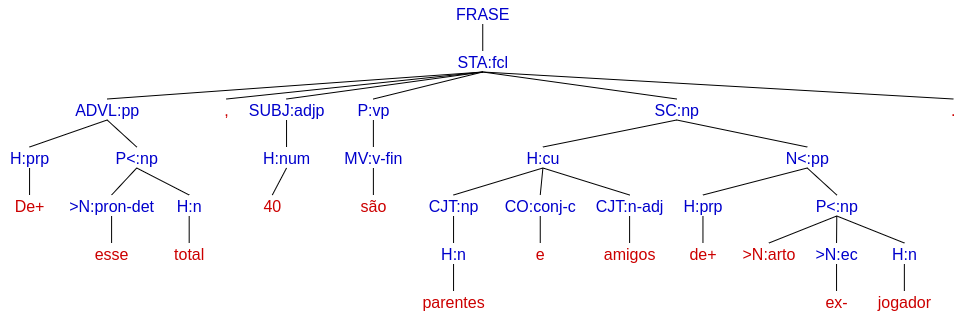
\includegraphics[width=\linewidth]{imagens/ec_bosque_ec_tree_orig.png}
        \caption{árvore original}
    % \end{subfigure}
    \end{minipage}
    % 
    \begin{minipage}{.45\textwidth}
        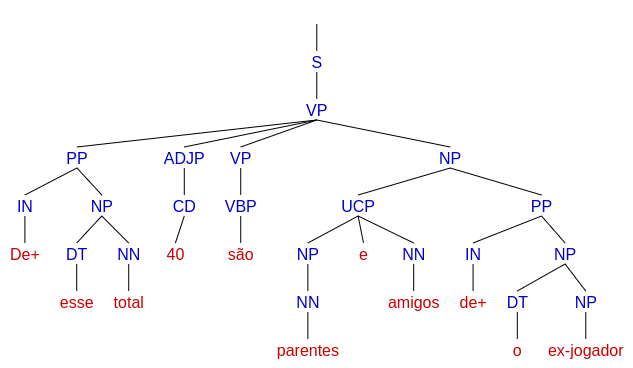
\includegraphics[width=\linewidth]{imagens/ec_bosque_ec_tree_trans.png}
        \caption{árvore transduzida}
    \end{minipage}
    \begin{minipage}{.45\textwidth}
        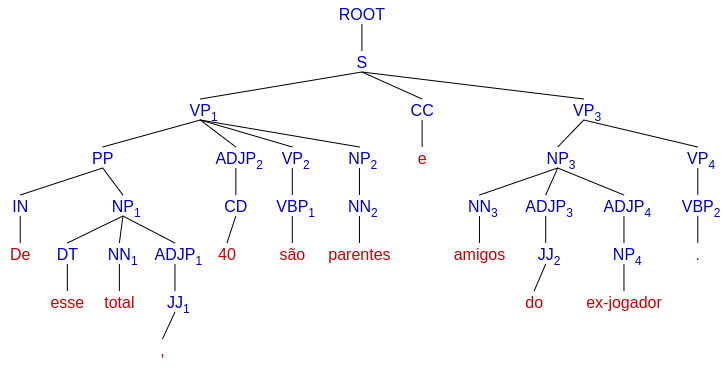
\includegraphics[width=\linewidth]{imagens/ec_bosque_ec_tree_ps.png}
        \caption{árvore gerada pelo SP}
    \end{minipage}
    % \begin{minipage}{.45\textwidth}
    %     \ldots
    %     \begin{tabbing}
    %         \=(NP\= (JJ ,) (NN Dawn)\+\\
    %         \>  (AD\=JP (JJ Upshaw)))\-\\
    %         \>(CC e)\\
    %         \>(VP\=\+\\
    %         \>  (VP (VBP Galina))\\
    %         \>  (NP\= (NN Gorchakova)\+\\
    %         \>      (ADJP (JJ .))))))))
    %     \end{tabbing}
    % \end{minipage}
    \caption[Estudo de caso BOSQUE - Sentença transduzida com \textit{ec}, e \textit{cu}]{Estudo da sentença CF866-2, \textquote{De esse total, 40 são parentes e amigos do ex-jogador.}, que possui a \textit{tag} \textit{ec}.}
    \label{fig:ec_bosque_ec_tree}
\end{figure}
\end{center}

A Figura \ref{fig:ec_bosque_ec_tree}
% vem com uma novidade inusitada: Foi considerada agramatical pelo \textit{parser} fatorado, disponibilizado pelo SP (que não abordamos neste trabalho). Mas foi interpretado pelo PCFG. 
traz um fato inesperado: a ideia com esta sentença era estudar a aplicação da \textit{tag} \textit{ec}, que inclusive não apresentou problemas. Mas a conjunção \textquote{parentes e amigos} foi desfeita pelo SP. \textquote{E} se tornou um mero irmão dos dois sintagmas, tal qual uma vírgula, e recebeu a \textit{tag} $CC$, que pouco aparece devido às conversões feitas na transdução para que o $SP$ aceitasse conjunções. O mesmo ocorre no \textit{parsing} da sentença CF318-C (fragmento em \ref{fig:ec_bosque_komp_detalhe}), mostrando que, apesar deste trabalho ter se guiado pelo \textit{Bracketing Guidelines} \cite{bracketing_ptb}, algumas estruturas poderiam se manter equivalentes às apresentadas no Bosque.

Outras análises serão apresentadas nos apêndices.